\documentclass[../main.tex]{subfiles}

\begin{document}

Una vez estudiados los circuitos RC y RL de primer orden en corriente continua y estado transitorio, podemos utilizar las expresiones de cada uno de los modelos matemáticos que los describen para implementar la simulación en una aplicación informática. Pero antes, debemos de hacer un estudio de las posibles tecnologías que nos permiten relizar esta implementación, pues dependiendo del tipo de aplicación, serán más convenientes unas tecnologías que otras.

\subsection{Tipos de aplicaciones según la compatibilidad}
Comenzamos el estudio de las tecnologías seleccionando el tipo de aplicación que más se ajuste a nuestras necesidades, dependiendo de la compatibilidad con los diferentes dispositivos del mercado. Distinguiremos entre tres grandes grupos de aplicaciones.


\begin{itemize}

    \item \textbf{Navitas}. Este tipo de aplicaciones son desarrolladas para ser lanzadas en una plataforma en específico. Debido a esto, una clara ventaja que presentan este tipo de \textit{software} es que, al estar diseñado para ser ejecutado en una arquitectura propia, su rendimiento respecto a los otros grupos en muy superior. Estas aplicaciones son útiles cuando se requiere un alto rendimiento y se quiere aprovechar el máximo de los recursos \textit{hardware} del sistema. Y en cuanto al coste, al tener que desarrollar el \textit{software} una vez por cada dispositivo con el que queramos que este sea compatible, se necesitará mayor tiempo de desarrollo y por lo tanto, un alto coste de producción.
    
    \begin{figure}[!h]
          \centering
          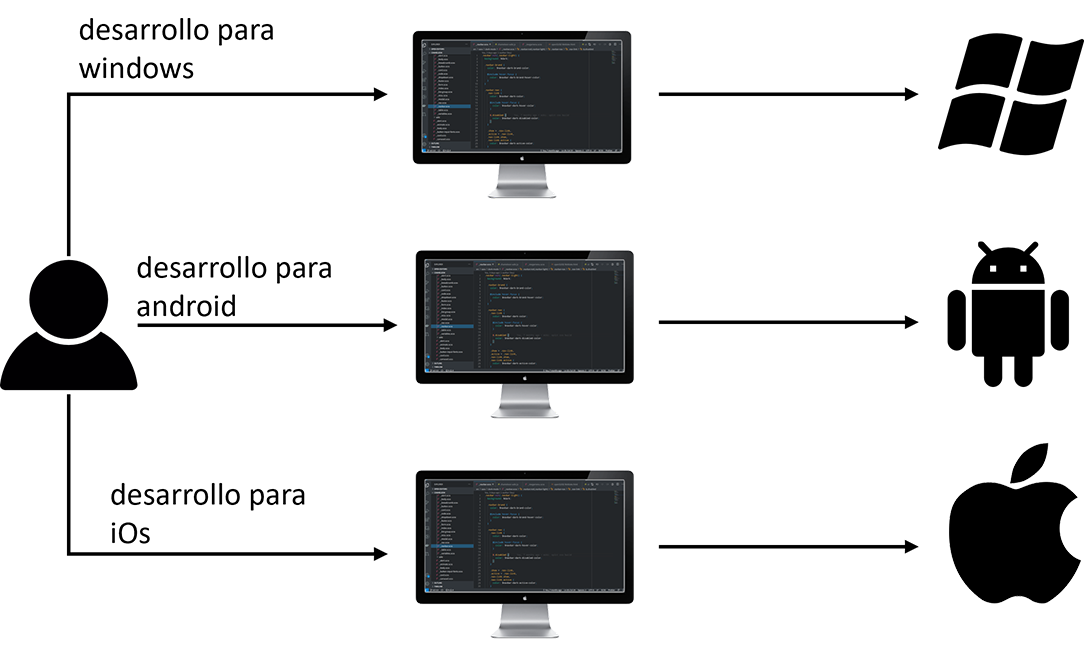
\includegraphics[width=0.7\textwidth]{images/aplicaciones_nativas.png}
          \caption{Aplicaciones Nativas}
          \label{fig:aplicaciones_nativas}
      \end{figure}
    
    \item \textbf{Híbridas}. En este segundo grupo encontramos aquellas aplicaciones que pueden ser ejecutadas en varias plataformas. Gracias a esto, la mayor parte de los dispositivos pueden hacer uso de estos programas, eso sí, el acceso a las funcionalidades del \textit{hardware} del dispositivo se encuentran más limitadas. Esto ocasiona un decremento en el rendimiento de la propia aplicación, por lo que la velocidad del \textit{software} aumentará o disminuirá dependiendo de las características del dispositivo.
    
    \begin{figure}[!h]
          \centering
          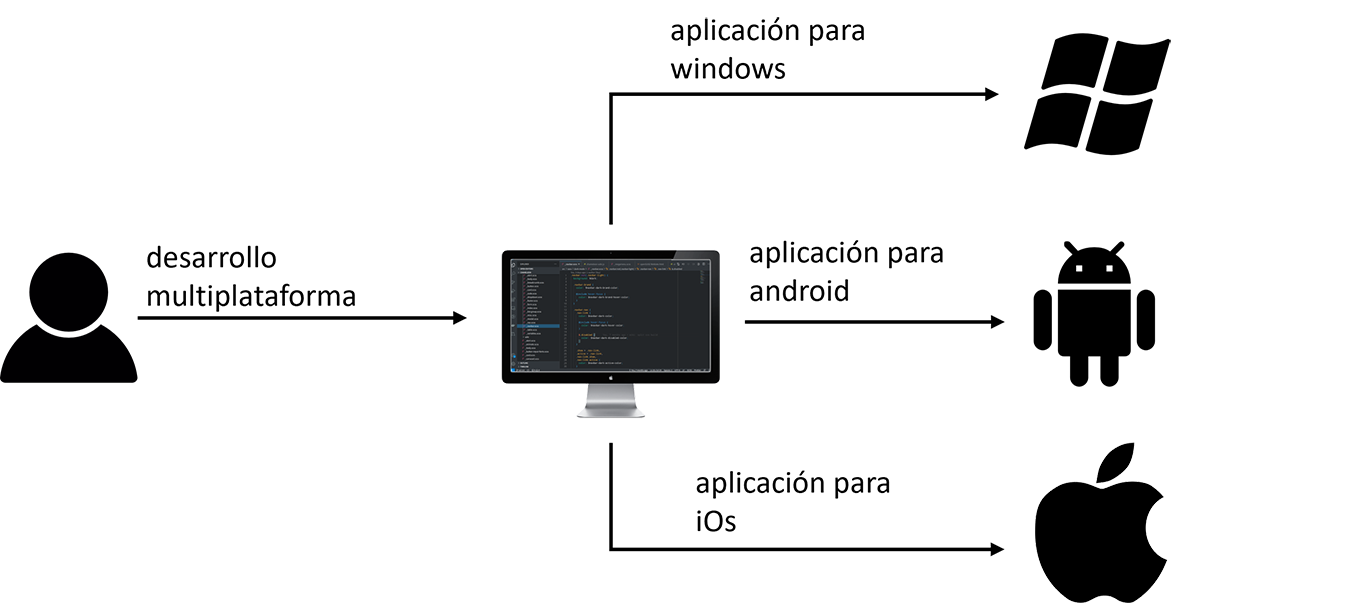
\includegraphics[width=0.8\textwidth]{images/aplicaciones_hibridas.png}
          \caption{Aplicaciones Híbridas}
          \label{fig:aplicaciones_hibridas}
      \end{figure}
    
    \item \textbf{Web}. Existe una estrecha correlación entre este grupo y el anterior, aunque las tecnologías utilizadas para su desarrollo no sean las mismas. Al igual que las \textit{aplicaciones híbridas}, las \textit{aplicaciones web} están orientadas a ser ejecutadas en varias plataformas. La única diferencia es que es necesario el uso de un navegador web para poder usarlas, y por lo tanto, requieren de conexión a internet. Esto puede resultar en una desventaja en caso de que se sufra una pérdida de conexión; sin embargo, tanto el coste de producción como el tiempo de desarrollo de este tipo de aplicaciones son muy inferiores respecto a los otros grupos. Al igual que ocurría con las aplicaciones híbridas, el acceso a características \textit{hardware} del dispositivo para la optimización del \textit{software} se encuentran muy limitado. Y en cuanto a niveles de rendimiento, las aplicaciones web se encuentran muy por debajo en relación a los otros dos grupos.
    
    \begin{figure}[!h]
          \centering
          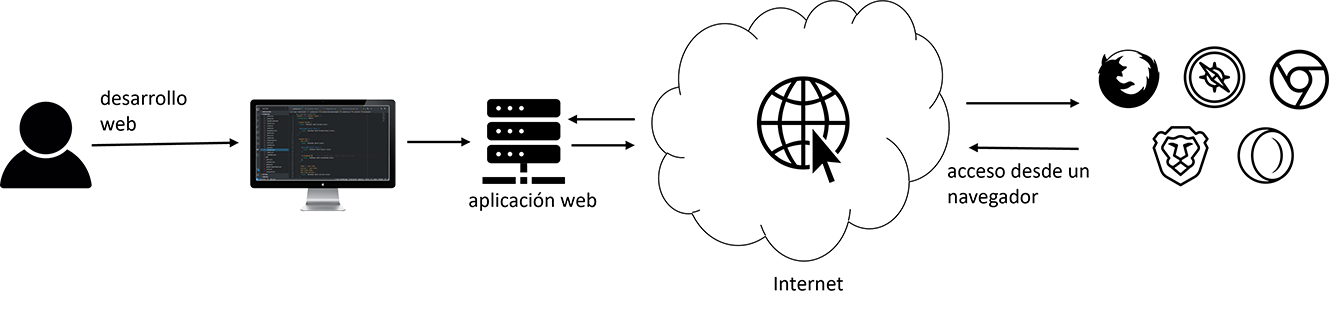
\includegraphics[width=\textwidth]{images/aplicaciones_web.png}
          \caption{Aplicaciones Web}
          \label{fig:aplicaciones_web}
      \end{figure}
    
    \end{itemize}
    
    Entre estos grupos, debemos de seleccionar aquél que se ajuste a nuestras necesidades. Es preferible que el \textit{software} que vamos a desarrollar sea accesible desde cualquier dispositivo, pues lo más probable es que los futuros usuarios no dispongan de una arquitectura específica para poder ejecutar la aplicación. Descartamos entonces las aplicaciones nativas. Otro punto importante a anlizar es el tipo de acceso. Por un lado, las aplicaciones híbridas obligan al usuario a descargar el programa e instalarlo en su dispositivo, obligando así un uso de memoria del mismo. Sin embargo, las aplicaciones web no requieren de dicha instalación y, además, pueden ser accesibles desde cualquier dispositivo que tenga instalado un navegador y por supuesto, una conexión a internet. Al tratarse de una simulación sencilla que no va a requirir un alto rendimiento y la potencia \textit{hardware} necesaria va a ser pequeña, el tipo de aplicación que más se ajusta a lo que estamos buscando son las \textit{aplicaciones web}.
    

    \subsection{La web y su evolución}
    Si tuviésemos que dar una definición de qué es Internet, diríamos que se trata de una red de intercambio de información cuyo propósito es la transmisión de datos por todo el mundo. Fue en 1963 cuando apareció el primer concepto de esta red bajo el nombre de \textit{ARPA} (\textit{Advanced Research Projects Agency}); un proyecto financiado por el departamento de defensa del gobierno norteamericano con el objetivo de establecer una comunicación descentralizada entre diferentes bases militares del país. No fue hasta seis años mas tarde cuando en la Universidad de California se consiguió dar un paso más allá, conectando entre sí dos ordenadores situados en diferentes universidades del país. \\
    
    El número de usuarios que utilizaban esta red en ese momento era de apenas unas miles de personas, y no fué hasta principios de la década de los 80 cuando el uso de esta red (conocida como \textit{ARPANET}) comenzó a extenderse al mundo gracias al lanzamiento del ISP (\textit{Internet Service Provider}), un servicio el cuál permitía a cualquiera con una dirección IP (\textit{Internet Protocol}) conectarse a esta red; alcanzando a principios de la década de los 90 a la cantidad de unas cien mil máquinas conectadas. Sin embargo esta fue reemplazada por una nueva red creada por la NSF (\textit{National Science Foundation}) a la que llamaron NSFNET y que inspiró a un grupo de científicos del CERN (\textit{Centro Europeo para la Investigación Nuclear} o \textit{Conseil Européen por la Recherche Nucléaire}) en la creación de lo que hoy día se conoce como la \textbf{Web}, con el objetivo de disponer de un sitio que alojase información y que fuese además accesible desde cualquier lugar del mundo.\\ 
    
    
    En su versión más primitiva, llamada la \textbf{web 1.0} \cite{web1.0}, las páginas eran fijas y no era común que estas se modificasen; además, estas páginas eran estáticas, careciendo completamente de interactividad. Para el renderizado de la web predominaba el uso de lo que comúnmente se llaman \textit{marcos} o \textit{framesets} utilizando una \textit{etiqueta} HTML con el mismo nombre. Por definición, una etiqueta o \textit{tag} en este lenguage de hipertexto es el nombre que reciben cada uno de los componentes con el que se estructura un documento HTML.
    
    
    Con ellas se establecía una estructura de diferentes marcos dentro de una página y, en cada uno de estos \textit{framesets} se ejecutaba un documento HTML diferente, obteniendo una modularización del documento principal. Otra característica relevante es el envío de los formularios. Mientras que hoy día esto se realiza mediante una serie de peticiones del protocolo HTTP (\textit{get}, \textit{post}, \textit{put}, ...) en ese momento la respuesta del formulario era enviada a través de un cliente de correo electrónico.\\
     
     \begin{figure}[!h]
          \centering
          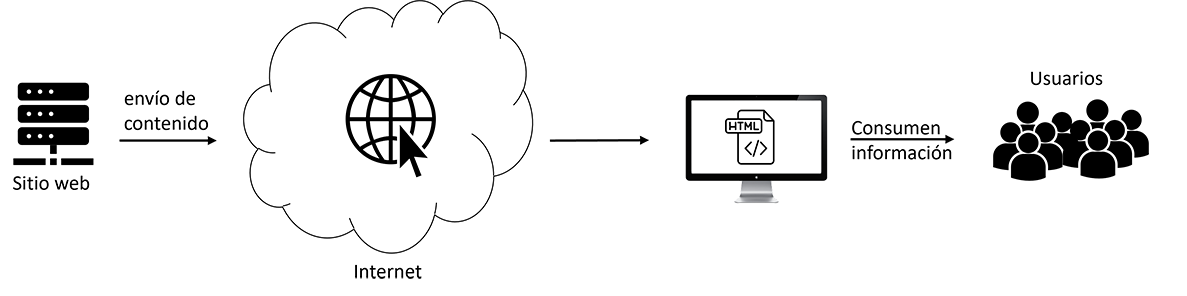
\includegraphics[width=\textwidth]{images/web1.0.png}
          \caption{La web 1.0}
          \label{fig:web1.0}
      \end{figure}
     
     La segunda fase de la web se inició con la aparición de las primeras páginas centradas en la distribución de recursos, es por eso que a esta se le conoce como la \textit{web social} o \textbf{web 2.0}. Ahora los sitios web no se encuentran limitados a mostrar información al usuario, sino que estos podrían añadir, editar, modificar, eliminar o compartir contenido con el resto de la comunidad, resultando ser las precursoras de las actuales redes sociales, blogs y wikis. A este nuevo grupo de páginas que permitían interactuar con ellas comienzan a llamarse \textit{aplicaciones web}, dejando el nombre de \textit{sitio} o \textit{página web} a las plataformas que ofrecían información no dinámica. Se introducen nuevas técnicas de formato para la estructura del documento, como CSS (\textit{Cascading Style Sheets}), AJAX (\textit{Asynchronous JavaScript and XML}) para el funcionamiento asíncrono de la web, uso de URLs semánticas que nos permiten entender cuál es el contenido que se va a consultar y el formato JSON (\textit{JavaScript Object Notation}) que es usado para dar estructura a los datos que se quieran transmitir entre servicios de una misma aplicación o como medio de comunicación con una API \cite{whatisAPI} (\textit{Application Programming Interface}).\\

     Actualmente esta versión de la web se encuentra en desarrollo, así que decimos que está en una \textit{beta} constante. En \textit{software}, nos referimos a beta como una de las primeras versiones del producto totalmente funcional, sobre las cuáles se realizan pruebas en sus funcionalidades y rendimiento. Además, el continuo lanzamiento de nuevas tecnologías permiten un desarrollo más acelerado de las aplicaciones web, las cuáles ofrecen un mayor rendimiento y una mejor experiencia para el usuario. 
     Sin embargo, mientras que la web 2.0 está en construcción, ya se está hablando de una nueva fase en la web. \\
    
     \begin{figure}[!h]
          \centering
          
\includegraphics[width=\textwidth]{images/web2.0.png}
          \caption{La web 2.0}
          \label{fig:web2.0}
      \end{figure}

    La \textbf{web 3.0} o \textit{web semántica} tiene su propósito en facilitar la navegación e indexación de las diferentes aplicaciones y sitios web, haciendo uso de técnicas avanzadas de análisis de datos e inteligencia artificial, consiguiendo así que la web se convierta en una BBDD (base de datos) mundial descentralizada. Cada uno de los usuarios de internet, dispondrá de un perfil único que usará para la autenticación de los diferentes servicios disponibles en la nube, creando así un espacio con mayor seguridad, privacidad, una experiencia personalizada durante la navegación en internet o mayor continuidad de los servicios (al tratarse de una red descentralizada, el número de interrupciones o cortes de conexión disminuirá). Pero esta nueva versión también podrá presentar una serie de desventajas: se requirirá de un hardware que ofrezca mayores prestaciones que sea capaz de soportar la transacción de mucha más cantidad de información, actualización de las diferentes aplicaciones y sitios actualmente desplegados o una nueva manera de protejer nuestros datos.  
    
    
    
    
    \subsection{Estructura de una aplicación web}
    
    Otro aspecto importante a tener en cuenta en el desarrollo, es la estructura base del proyecto. Si bien el lenguaje de programación puede facilitar y ayudar en la implementación, la buena definición de una estructura puede favorecer al desarrollo de la misma. Aunque la base de una aplicación de este tipo no se está bien definida y existe cierta libertad en su configuración y organización, podemos establecer un modelo generalista que divide internamente una aplicación web en tres capas bien diferenciadas.
    
    \begin{itemize}
        \item La primera de las capas llamada \textbf{capa de datos} o \textbf{capa lógica} es la parte más abstracta e interna de la aplicación. En ella definiremos el esqueleto principal de cómo organizar nuestros datos y archivos multimedia.
        
        \item Por encima encontramos la llamada \textbf{capa de negocio}. En esta, se implementa toda la lógica necesaria que permite interactuar con la \textit{capa lógica}, como por ejemplo añadir, eliminar o modificar contenido de la misma. Se trata de un gestor de información encargado de la comunicación entre la \textit{capa de datos} y el usuario de la aplicación, quién hace uso de la llamda \textit{capa de presentación}. A este gestor también se le conoce como \textit{middleware}.
                
        \item En el nivel más alto, tenemos la \textbf{capa de presentación}. Mientras que las dos anteriores se ejecutan en el lado oculto de la aplicación (lo que llamaremos servidor), esta lo hará en el lado visible de la misma (cliente). En ella se hace una interpretación de las diferentes peticiones de los usuarios haciendo uso de las operaciones implementadas en la \textit{lógica de negocio}. Las acciones que un usuario puede hacer dependerá de entre otras cosas del diseño y restricciones que se presenten en esta capa.
        
        
      
    \end{itemize}
    
    \begin{figure}[!h]
          \centering
          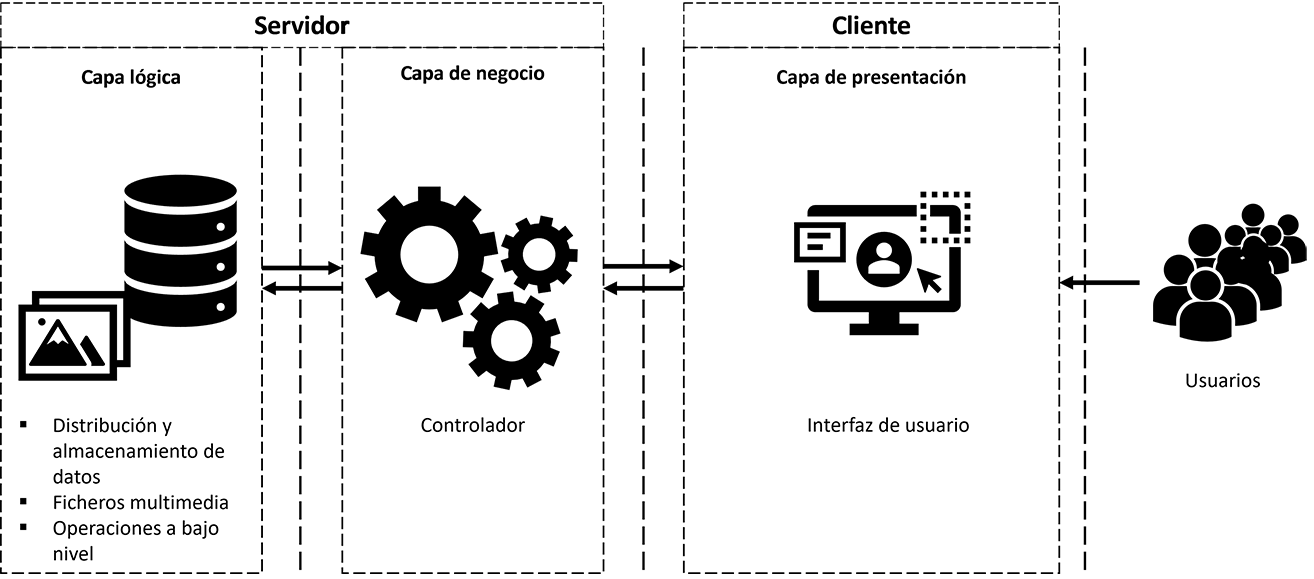
\includegraphics[width=\textwidth]{images/estructura_aplicacion_web.png}
          \caption{Aplicación web por capas}
          \label{fig:web_capas}
      \end{figure}
      
    Para simplificar aún más esta división por capas, podemos añadir un nivel más de abstracción. Este se basa en diferenciar las dos partes de la aplicación que están interactuando entre sí. Como se puede observar en la figura \ref{fig:web_capas}, el usuario actúa directamente con la interfaz gráfica, ignorando completamente todo lo que ocurre por detrás: distribución y almacenamiento de los datos, operaciones a bajo nivel, procedimientos ejecutados en el controlador de la capa de negocio, ... Nombraremos entonces a todas aquellas capas que interactúen de forma directa con el usuario como \textbf{front-end} de la aplicación mientras que, todo lo que sea ajeno a él será el \textbf{back-end}. \\
    
    Esta división nos permite agilizar el proceso de desarrollo, así como facilitar el despliegue de la aplicación. Por un lado, como se vió en el primer capítulo, el ciclo de vida del \textit{software} consta de varias etapas y una de ellas es la fase del \textit{diseño}. En ella se llevará a cabo la construcción a muy alto nivel de cada una de las capas de la aplicación, como por ejemplo la nomenclatura de las acciones en el controlador o la organización de los datos dentro de la BBDD. Si el diseño es lo bastante bueno y se encuentra bien documentado, deberíamos de ser capaces de desarrollar a la par el \textit{back-end} y el \textit{front-end}, pues al tratarse de módulos independientes y al usar un conector común, basta con que éste se encuentre bien definido. 
    
    En cuanto al despliegue, al tener separados en dos bloques diferentes la parte del cliente y del servidor, cada uno de los módulos pueden estar funcionando en \textit{hosts} diferentes, teniendo así una aplicación web descentralizada. Esto no se aplica solamente a estas dos partes, sino también a cada una de las capas que forman el \textit{back-end} y el \textit{front-end}. \\
    
    En la figura \ref{fig:web_despliegue} podemos observar un diagrama con el despliegue de una aplicación web descentralizada. Disponemos de un un \textit{host} para el despliegue de cada una de las capas. Para enlazar cada una de ellas como vemos en la figura \ref{fig:web_capas}, basta con conectarlas a internet y dentro de cada una configurarlas para que redireccionen las peticiones a la capa correspondiente. Por ejemplo, tenemos en la nube una aplicación web basada en una enciclopedia sobre historia. Ahora, un usuario quiere añadir una entrada a esta wiki así que cuando entra al navegador y utiliza la URL de la aplicación, este accede a la dirección del servidor que contiene la capa de presentación. Si añade una entrada, la capa de presentación se comunica con el controlador a través de internet y este, con la capa lógica de igual manera. El usuario no necesita conocer dónde se alojan las capas de negocio o lógica (\textit{back-end}) pero sí que puede acceder a la interfaz de usuario y utilizarla para añadir una nueva sección en la enciclopedia (\textit{front-end}).\\
 
    \begin{figure}[!h]
          \centering
          
\includegraphics[width=\textwidth]{images/despliegue_web.png}
          \caption{Diagrama de una aplicación web}
          \label{fig:web_despliegue}
      \end{figure}
    
    Y esto se puede complicar todo lo que deseemos. Podemos añadir una nueva capa de datos con su respectivo controlador de tal forma que tengamos dos servicios diferentes en una misma aplicación, distribuir el almacenamiento por varios puntos geográficos (por ejemplo, uno para datos y otro para fotos y videos) y unificar estos directorios como uno solo o tener varios controladores para una misma capa lógica.\\
    
    
    Con esto hemos visto una idea general de cómo se puede organizar una aplicación web. Sin embargo, para la implementación de las simulaciones no va a ser necesario montar este tipo de infraestructura. En primer lugar, el almacenamiento de datos no va a ser necesario ya que los resultados que se van a generar serán meramente informativos para el usuario. Puesto que vamos a prescindir de una base de datos, tampoco necesitaremos de un controlador que se encargue de actualizar constantemente la información guardada. Solamente nos queda centrarnos en el \textit{front-end} de la aplicación, reduciendo considerablemente el desarrollo del \textit{software}. Pero antes, debemos de barajar todas las tecnologías posibles que nos ayuden en la implementación.
    
    
    \subsection{Tecnologías \textit{front-end}}
    Antes de ralizar un estudio de las posibles tecnologías en profundidad, la primera tecnología considerada para la implementación de las simulaciones fue la elaboración de un \textit{applet}. Un \textbf{applet} \cite{aplicacionesyapplets} es un \textit{software} o programa de ordenador escrito en el lenguaje de programación \textit{Java}. Estos se podían añadir a un documento HTML y, gracias a la \textit{JVM} o \textit{Java Virtual Machine} ejecutarlos en el navegador del cliente. El uso de este tipo de \textit{software} se extendió rápidamente ya que al poder ejecutarse en cualquier dispositivo independientemente del sistema operativo y navegador, permitía a cualquier usuario ver el contenido que le proporcionaba el applet. Esta es la definición de lo que conocemos como una \textit{aplicación multiplataforma}.
    
    \begin{figure}[!h]
          \centering
          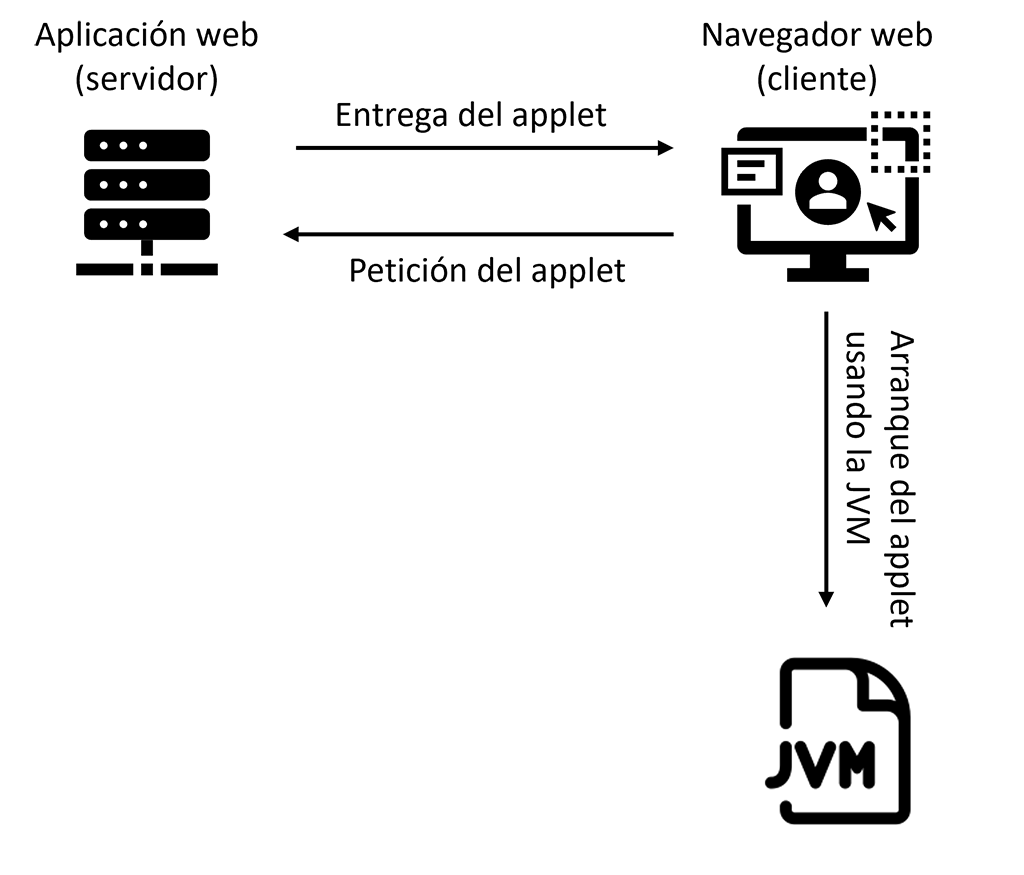
\includegraphics[width=0.55\textwidth]{images/arranque_applet.png}
          \caption{Arranque de un applet incrustado en una página web.}
          \label{fig:arranque_applet}
      \end{figure}
     
    Pero con el tiempo comenzarían a aparecer vulnerabilidades en este tipo de aplicaciones que afectarían directamente a la JVM y posteriormente al sistema, exponiendo al usuario a ser víctima de ciberdelincuentes, en ataques de \textit{ransomware} (técnica utilizada para encriptar los ficheros del sistema, denegando el acceso al propietario y pidiendo posteriormente un pago por su desbloqueo) o mediante la instalación de \textit{malware} (se trata de un software malicioso cuyo principal objetivo es dañar cualquier dispositivo o red). Es por es que hoy día navegadores como \textit{Chorme} o \textit{Firefox} no estén habilitados para ejecutar \textit{applets}, aunque existen otros que lo permiten si se hace el uso de ciertos \textit{plugins}; es decir, programas cuyo objetivo es extender la funcionalidad de otro software sin necesidad de modificarlo desde código.\\ 
    
    
    Algunas de las ventajas que presentaban este tipo de programas informáticos eran objetos animados e interactivos, reproducción de sonidos, implementación de funciones encargadas de proyectar los gráficos del \textit{applet} correctamente o la visualización de gráficas y diagramas. Ya que carece de sentido utilizar este tipo de software por estar prácticamente obsoleto, usaremos algunas de las nuevas herramientas introducidas con la \textit{web 2.0}, como \textit{CSS} o \textit{JavaScript}.
    
    
    \subsubsection{HTML}
    Creado en 1991 por Tim Berners-Lee, HTML (del acrónimo anglosajón \textit{HyperText Markup Languaje}) es un lenguaje basado en etiquetas utilizado para definir la estructura de las páginas web. En su primera versión se disponía de unas dieciocho  etiquetas las cuáles nos permitían añadir elementos de vídeo, texto o imágenes; y que hoy día con la  versión de HTML5, el número de estas etiquetas asciende a más de 130. La definición de estos elementos se realiza encerrando entre corchetes el nombre del componente que queramos añadir y que en ocasiones se les puede agregar atributos. También es posible encontrar etiquetas que no necesitan de un elemento de cierre, como es el caso de la línea horizontal (\textit{hr}) o el salto de línea (\textit{br}). 
    
    
    \begin{figure}[!h]
        \centering
        \begin{minted}[
            frame=lines,
            framesep=2mm,
            baselinestretch=1.2,
            bgcolor=LightGray,
            fontfamily=\familydefault,
            fontsize=\footnotesize,
            linenos
        ]{html}
        
        <nombre-etiqueta atributo1="valor_atributo_1" atributo2="valor_atributo_2"> ... </nombre-etiqueta>
        
        \end{minted}
        \caption{Definición etiqueta HTML.}
        \label{fig:definicion_etiqueta_html}
    \end{figure}
    
    La estructura elemental de un documento HTML queda definida por la declaración de los siguientes elementos:

    \begin{itemize}
        \item En primer lugar tenemos la sección \textbf{head} o cabecera de la página. En ella se define la información necesaria que describe el contenido del documento HTML, como por ejemplo, establecer el título que aparece en la pestaña del navegador, formato del texto a incluir el documento (codificación de los caracteres como UTF-8) o los diferentes enlaces que nos permitan acceder a \textit{scripts} y \textit{hojas de estilos} ya sea de manera local como remota. Su definición no es obligatoria.
        
        \item Como segundo grupo tenemos el cuerpo de la página (\textbf{body}). En él vamos a definir todo el contenido que va a ser visualizado en el navegador. Solamente se puede definir uno por documento.
    
    \end{itemize}
    

    
    \begin{figure}[!h]
        \centering
        \begin{minted}[
            frame=lines,
            framesep=2mm,
            baselinestretch=1.2,
            bgcolor=LightGray,
            fontfamily=\familydefault,
            fontsize=\footnotesize,
            linenos
        ]{html}
        
        <!DOCTYPE html>
        <html>
            <!-- Cabecera de la página -->
            <head>
                <!-- Definición de metadatos  -->
                <meta name="language" content="es" > 
                <meta name="description" content="descripción del sitio" > 
                <!-- Título de la página -->
                <title> Título </title>
                <!-- Enlace a ficheros de script  -->
                <script src="ruta-del-script" type="tipo-de-script"></script>
                <!-- Enlace a ficheros de hoja de estilos  -->
                <link rel="stylesheet" href="ruta-de-hoja-estilos" >
            </head>
            
            <!-- Cuerpo de la página -->
            <body>
                <!-- Párrafo de cabecera. Va desde h1 hasta h6 (más a menos importancia) -->
                <h1> ... </h1>
                <!-- Párrafo de texto -->
                <p> ... </p>
                <!-- Sección de un documento -->
                <div> ... </div>
                ...
            </body>
        </html>
        
        \end{minted}
        \caption{Ejemplo muy básico de la definición de un documento HTML. Además de las mostradas, existen más elementos que pueden utilizarse cada cuál tiene sus propios atributos. En \cite{etiquetasbasicashtml} se definen con más detalle cada una de las etiquetas del ejemplo además de otras que no aparecen.}
        \label{fig:estructura_documento_html_I}
    \end{figure}

    
    Sin embargo, todo lo que podemos hacer con HTML está limitado a aquello que ya se encuentra definido por las diferentes etiquetas y atributos que este lenguaje nos proporciona. Así que para dar forma a esta estructura y hacerla más atractiva para el usuario, utilizaremos lo que se conoce como una hoja de estilos.

    
    \subsubsection{CSS y Bootstrap}
    Definimos como una \textit{hoja de estilos} a aquellos ficheros utilizados en la definición de los formatos de elementos HTML, cuya principal finalidad es mejorar tanto el aspecto visual como el diseño de los mismos. Para ello hacemos uso de \textbf{CSS} o \textit{Cascading Style Sheets}. Se trata de un lenguaje de programación basado en la definición de atributos mediante el uso de \textit{selectores}. Un selector es la unión que se encarga de vincular el elemento HTML definido en el documento web con el estilo definido. Esto nos permite aplicar formatos a diferentes objetos que se rijan por un mismo selector, como el uso de un identificador o mediante algún atributo espécifico de dicho elemento.  En \cite{selectoresCSS} se puede ver con más detalle los selectores existentes acompañados de ejemplos. \\
 
    
    Otra característica importante es que la definición de estos estilos se puede realizar de dos formas diferentes. La primera de ellas es mediante el uso de una etiqueta \textit{style} en la cabecera del documento. Entre el nombre de  de apertura y de cierre se definen todas las modificaciones que se quieran hacer a los elementos de nuestra página web utilizando los selectores previamente vistos, con la inconveniencia de que los estilos definidos solamente pueden ser aplicados a elementos de la misma página. Así que para evitar este problema, la opción más eficaz y que nos permite la modularización de código y por consiguiente una mejor organización del mismo, es definir nuestra hoja de estilos en un fichero independiente. Esto nos permite definir una serie de estilos que pueden ser reutilizados en varios documentos HTML, mediante el uso de la etiqueta \textit{link} tal y como se puede observar en el código de la figura \ref{fig:estructura_documento_html_I}.\\ 
    
    Aunque estos sean los dos métodos más utilizados, existe un tercero que puede llegar a carecer de utilidad si lo que se quiere conseguir es un código limpio y organizado. A cada objeto HTML se le puede agregar en su \textit{tag} de apertura un atributo llamado \textit{style}. La función de este es incluir un formato a dicho elemento. En cambio, se puede sacar provecho de este atributo si el diseño a aplicar es muy puntual y simple y además queremos evitar conflictos con elementos similares. Aunque sin duda alguna, la segunda opción es la más adecuada.\\
    
    El uso de selectores no es complejo mientras que el diseño de la interfaz gráfica sea sencillo. Si se quiere elaborar una interfaz un poco más compleja, el nivel de dificultad de CSS se incrementa bastante, convirtiendo la creación de los estilos de la página web en un trabajo complicado. Para facilitar su elaboración, podemos hacer uso de una serie de módulos ya creados que nos permite dar a nuestros elementos HTML formatos ya elaborados a los  que posteriormente se les pueden cambiar el aspecto. Una de estas herramientas es \textbf{bootstrap}.\\
    
    Creada por Mark Otto y Jacob Thornton, \textit{bootstrap} surge como una biblioteca usada en el diseño e implementación de las UI (\textit{Users Interfaces} o interfaces de usuario) de Twitter y no fué hasta 2011 cuando este proyecto se cataloga como software \textit{open-source} o de código abierto. Un software es de código abierto cuando este es de dominio público y su código fuente puede ser descargado y utilizado para agregar nuevas funciones, corregir problemas de seguridad o simplemente realizar una optimización del mismo. Además, el software modificado puede volver a distribuirse siempre que esta sea bajo la misma licencia. La principal característica por la que se conoce a este \textit{framework} es la consistencia que se añade a la página web. Existen un número bastante alto de selectores de clase ya definidos para la creación de botones, deslizadores, \textit{inputs} de datos o barras de navegación que permiten a los desarrolladores utilizar una nomenclatura en común y facilitar así el desarrollo de la aplicación. Pero por lo que realmente se caracteriza \textit{bootstrap} es en favorecer en la construcción de \textit{webs responsive}, o lo que es lo mismo, permite redimensionar la web dependiendo del dispositivo sobre el que se esté utilizando, teniendo que producir una nueva vista adaptado al dispositivo en cuestión.\\
    
    En el caso de la aplicación que vamos a desarrollar solamente vamos a contemplar aquellos dispositivos útiles que permitan al alumno una mejor visualización de los resultados de las simulaciones, como pueden ser un portátil o una tableta. Por ello, se tendrán en cuenta las pantallas cuya resolución sea mayor a diez pulgadas o con un ancho que supere los 1280 píxeles para evitar que los elementos de la ventana se colapsen entre ellos. En caso de querer adaptarlo para otros dispositivos (móvil u otras pantallas especiales), habrá que rediseñar e implementar la interfaz de usuario ajustadas a estos equipos.
    

    \subsubsection{JavaScript}
    JavaScript (JS) es un lenguaje de programación \textit{script} e \textit{interpretado} creado por Brendan Eich bajo el nombre de \textit{Mocha}, en su trabajo por añadir nuevas funcionalidades al navegador web Netscape, además de tratar de mejorar las ya existentes \cite{elocuentJS}. Con una sintaxis heredada de \textit{C++} y \textit{Java}, JavaScript está habilitado para la programación orientada a objetos e incluso tiene variantes que permiten el tipado de sus funciones y variables (\textit{TypeScript}). \\
    
    \begin{figure}[!h]
        \centering
        
\includegraphics[width=\textwidth]{images/arbol_dom_ejemplo.png}
        \caption{Ejemplo de árbol DOM}
        \label{fig::arbol_dom_ejemplo}
    \end{figure}
    
    Considerado como el lenguaje por excelencia de la programación web, una de las principales características de JS es la creación de scripts sencillos que permiten dinamizar los documentos HTML mediante la modificación de sus elementos. Para ello, se hace uso del \textit{DOM} o \textit{Document Object Model}. Se trata de una estructura de nodos organizados jerárquicamente (árbol) en la que se incluye el contenido del sitio web; es decir, estructura del documento HTML con sus respectivos estilos en CSS. Todos estos árboles tienen un elemento raíz que hace referencia al documento sobre el que se va a ejecutar dicho script (\textit{document}), del cuál se extienden el resto de elementos. Además, para poder interactuar con este árbol de una manera más fácil, JavaScript tiene integrado una API que nos permite acceder, modificar, crear o eliminar elementos \cite{javaScriptDOM}. Podemos ver en la figura \ref{fig::arbol_dom_ejemplo} el árbol DOM correspondiente al código HTML de la figura \ref{fig:estructura_documento_html_I}.\\
    
    Otra de las características de este lenguaje es que es interpretado. La ejecución de programas escritos en otros lenguajes de programación como \textit{C++}, \textit{Haskell} o \textit{Fortran} sucede gracias a la intervención de un programa compilador que se encarga de traducir el código fuente escrito a código máquina, siendo este último el consumido por el procesador, ofreciendo cualidades como una mejor velocidad, eficiencia y robustez. Luego, un lenguaje interpretado es aquel cuyos programas se ejecutan instrucción a instrucción directamente mediante el uso de un intérprete sin necesidad de ser traducido a código máquina en un paso intermedio. Aunque los lenguajes interpretados suelen ser más lentos en ejecución que los compilados, ofrecen ventajas como la de poder ser ejecutados en cualquier plataforma o aumentar el rendimiento de la aplicación; pues lenguajes como JavaScript al estar diseñados para ser utilizados en el servicio del cliente, disminuyen la carga en el servidor. \\
    

    Aunque JavaScript sea un lenguaje de programación fácil de aprender y además se dispone de una API nativa que facilita la interacción con los documentos HTML, cuando la aplicación que queremos desarrollar es demasiado compleja la mejor opción a la que podemos recurrir es a utilizar un \textit{framework} de desarrollo; al igual que ocurría con \textit{bootstrap} para acelerar la creación de estilos CSS. Existen muchos \textit{frameworks} \textit{front-end} escritos con JavaScript, como pueden ser \textit{Vue.js}, \textit{Angular}, \textit{Svelte}, \textit{ReactJS} o \textit{jQuery} entre otros. Cada uno de ellos presentan sus respectivas ventajas frente al resto aunque, si tuviésemos que elegir por relación entre dificultad de aprendizaje y velocidad de desarrollo, \textit{ReactJS} sería el entorno más adecuado.
    

    \subsubsection{ReactJS}
    

    ReactJS es un conjunto de librerías \textit{open source} escritas en JavaScript y que utiliza NodeJS como entorno de ejecución. Una de las características que definen a este \textit{framework} de programación, es que permite el desarrollo de interfaces de usuario para la web basadas en \textit{single-page}. \\
    
    Mientras estamos navegando por una aplicación web en busca de información y durante la navegación tiene lugar una actualización de su contenido, normalmente seguiremos viendo la información sin esas modificaciones. Para renderizar el nuevo contenido debemos de realizar una recarga de la página, durante la cual se realiza una petición para obtener la nueva información ya actualizada. Sin embargo, las aplicaciones web que utilizan la tecnología de \textit{single-pages} no necesitan realizar esta recarga de la página, ofreciendo así una mejor experiencia de usuario. Estas utilizan AJAX (\textit{Asynchronous JavaScript and XML}), una técnica que permite recargar solamente aquellas partes de la web que han sufrido cambios; que en el caso de este \textit{framework} estos cambios se producen por la actualización independiente de los \textbf{componentes} de la página, facilitando así tanto la implementación como el renderizado de la misma. Algunos ejemplos de aplicaciones \textit{single-page} son: Gmail, Google Maps o Paypal. \\
    
    Un componente en React es la definición de cualquier objeto que queramos incluir en nuestra interfaz de usuario, como puede ser un párrafo de texto, una imágen, ... o elementos algo más complejos como un menú de navegación. La ventaja que estos presentan es que pueden ser reutilizados en cualquier parte del código, ahorrando así tiempo en la implementación. 
    
    Cualquier componente definido en React, consta de tres estados: inicialización (\textit{mounting}), actualización (\textit{updating}) y destrucción (\textit{unmounting}).
    
    \begin{figure}[!h]
        \centering
        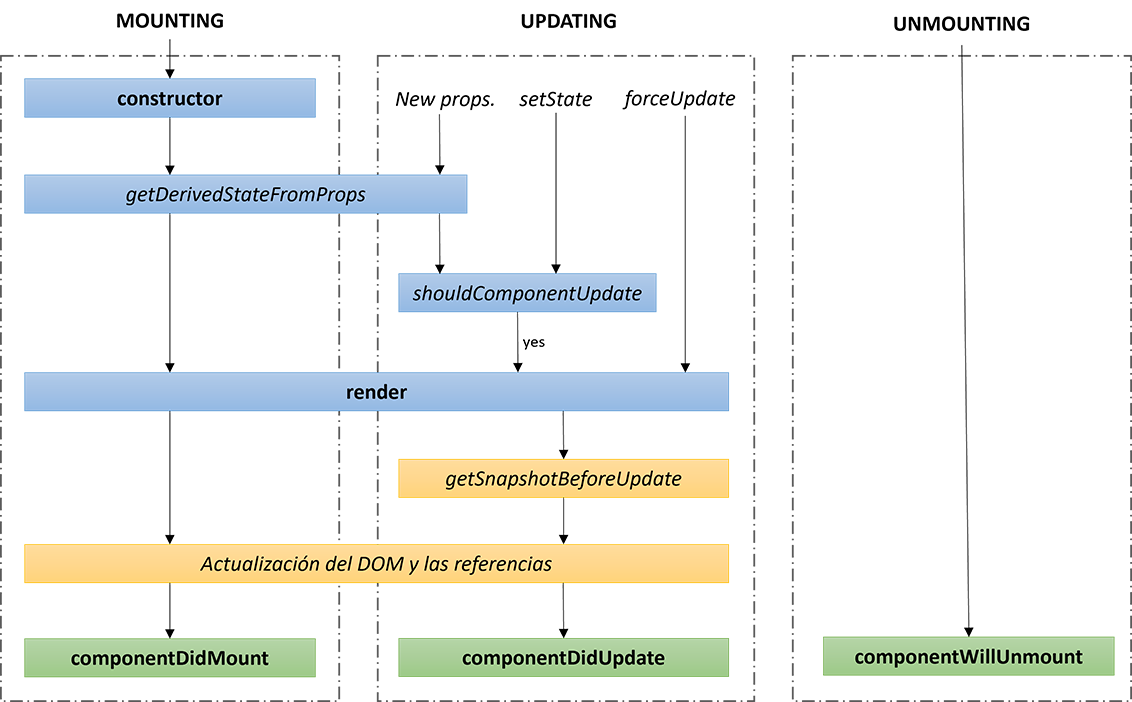
\includegraphics[width=\textwidth]{images/react_component_lifecycle.png}
        \caption{Ciclo de vida de un componente en ReactJS \cite{reactComponent}}
        \label{fig::react_component_lifecycles}
    \end{figure}
    
    En primer lugar tenemos la etapa de \textit{mounting}, que abarca desde la inicialización del componente con unas propiedades y estado predeterminados hasta que es renderizado y mostrado al usuario por primera vez. La linea que sigue esta etapa es la siguiente: 
    
    
    \begin{itemize}
        \item  En la mayoría de lenguajes que permiten la programación orientada a objetos (POO), existe un método llamado \textbf{constructor} que se encarga de inicializar el objeto cuando se crea una instancia de él. En el caso de un componente de React, los propósitos del constructor son la creación del estado local del componente así como ligar las funciones asociadas a la captura de eventos a una variable (también conocido como \textit{binding}). En caso de que no sea necesario hacer ninguna de estas operaciones, la definición del constructor se puede omitir.
        
        \item A continuación, se invoca un método llamado \textbf{getDerivedStateFromProps}, el cuál se invoca justo antes del renderizado del componente. Este es rara vez utilizado, y su principal objetivo es cambiar el estado local del componente cuando las propiedades (\textit{props}) iniciales son modificadas. El uso de este procedimiento no es obligatorio cuando los valores de las \textit{props} no cambian.

        
        \item Una vez creada la instancia del componente y establecido un estado inicial del mismo, lo siguiente que ocurre es la renderización del componente mediante el método \textbf{render}. Para ello se hace uso de JSX, una extensión de JavaScript que permite la definición de los componentes utilizando un lenguaje de hipertexto similar a HTML al que se le añade la potencia de JavaScript para personalizarlos. La sintaxis de JSX es igual a la de HTML, solo que además de poder utilizar las etiquetas predeterminadas de este lenguaje, también podemos añadir nuevas etiquetas con el nombre de un componente que hayamos creado.
        
        Ya montado el componente, este se actualiza en el DOM y justo después se ejecuta el método \textbf{componentDidMount}. Normalmente este procedimiento es utilizado para extraer datos de una API o realizar algunas modificaciones del estado local. Su definición no es obligatoria.
        
    \end{itemize}
    
    Por otro lado tenemos la etapa de \textit{updating} o actualización, la cuál podría decirse que es la etapa del ciclo en la que más tiempo pasa un componente; pues cada vez que hagamos una modificación en alguna de las propiedades, cambiemos el estado local o forcemos una actualización (\textit{refresh}), se llevará a cabo una nueva renderización (\textit{re-render}). 

    \begin{itemize}
        \item Como vemos en el diagrama de la figura \ref{fig::react_component_lifecycles}, la actualización de un componente ocurre por los tres motivos comentados en la línea anterior. En caso de que se actualicen las \textit{props} se llama obligatoriamente al procedimiento \textit{getDerivedStateFromProps} ya descrito, y luego, en caso de que el componente deba de actualizarse, este se vuelve a renderizar. En cambio, si lo que modificamos es el estado o forzamos la actualización se invoca directamente el procedimiento encargado en la renderización del objeto.
        
        En caso de que el componente no deba de actualizarse, simplemente esta etapa del ciclo finaliza y volvemos al inicio de ella (\textit{shouldComponentUpdate}).
        
        \item Justo después se invoca \textbf{getSnapshotBeforeUpdate}, un método cuyo objetivo es capturar información sobre el DOM antes de que este cambie, aunque no suele utilizarse. Un ejemplo de uso lo podemos ver en \textit{WhatsApp}, si tuviésemos que programar la interfaz en React. Cuando recibimos un nuevo mensaje de uno de nuestros contactos, justo encima de él observamos que aparece una alerta de que tenemos una nueva notificación. Para mostrar esta alerta (la cuál no es necesaria de guardar en el historial de mensajes), se toma la posición de \textit{scroll} del último mensaje recibido, se inserta esta alerta y después el nuevo mensaje. Cuando ya hemos visto el mensaje, simplemente eliminamos esta alerta actualizando de nuevo la posición de \textit{scroll}.
        
        \item Por último se actualiza el DOM y, posteriormente, se llama al procedimiento \textbf{componentDidUpdate}, cuyo objetivo es el mismo que el método \textit{componentDidMount}, solo que en este caso se ejecuta cada vez que se actualiza el componente. 
        
    \end{itemize}
    Por último tenemos la fase de \textit{unmounting} o destrucción del componente. Esta etapa comienza cuando el componente en cuestión es eliminado del DOM de la página, invocando así el método \textbf{componentWillUnmount}, el cuál puede ser utilizado para limpiar o cancelar peticiones a una base de datos, invalidación de temporizadores (como por ejemplo en funciones que se ejecutan cada cierto tiempo) o eliminar registros creados en la etapa de \textit{mounting} con el método \textit{componentDidMount}.\\
    
    \begin{figure}[!h]
        \centering
        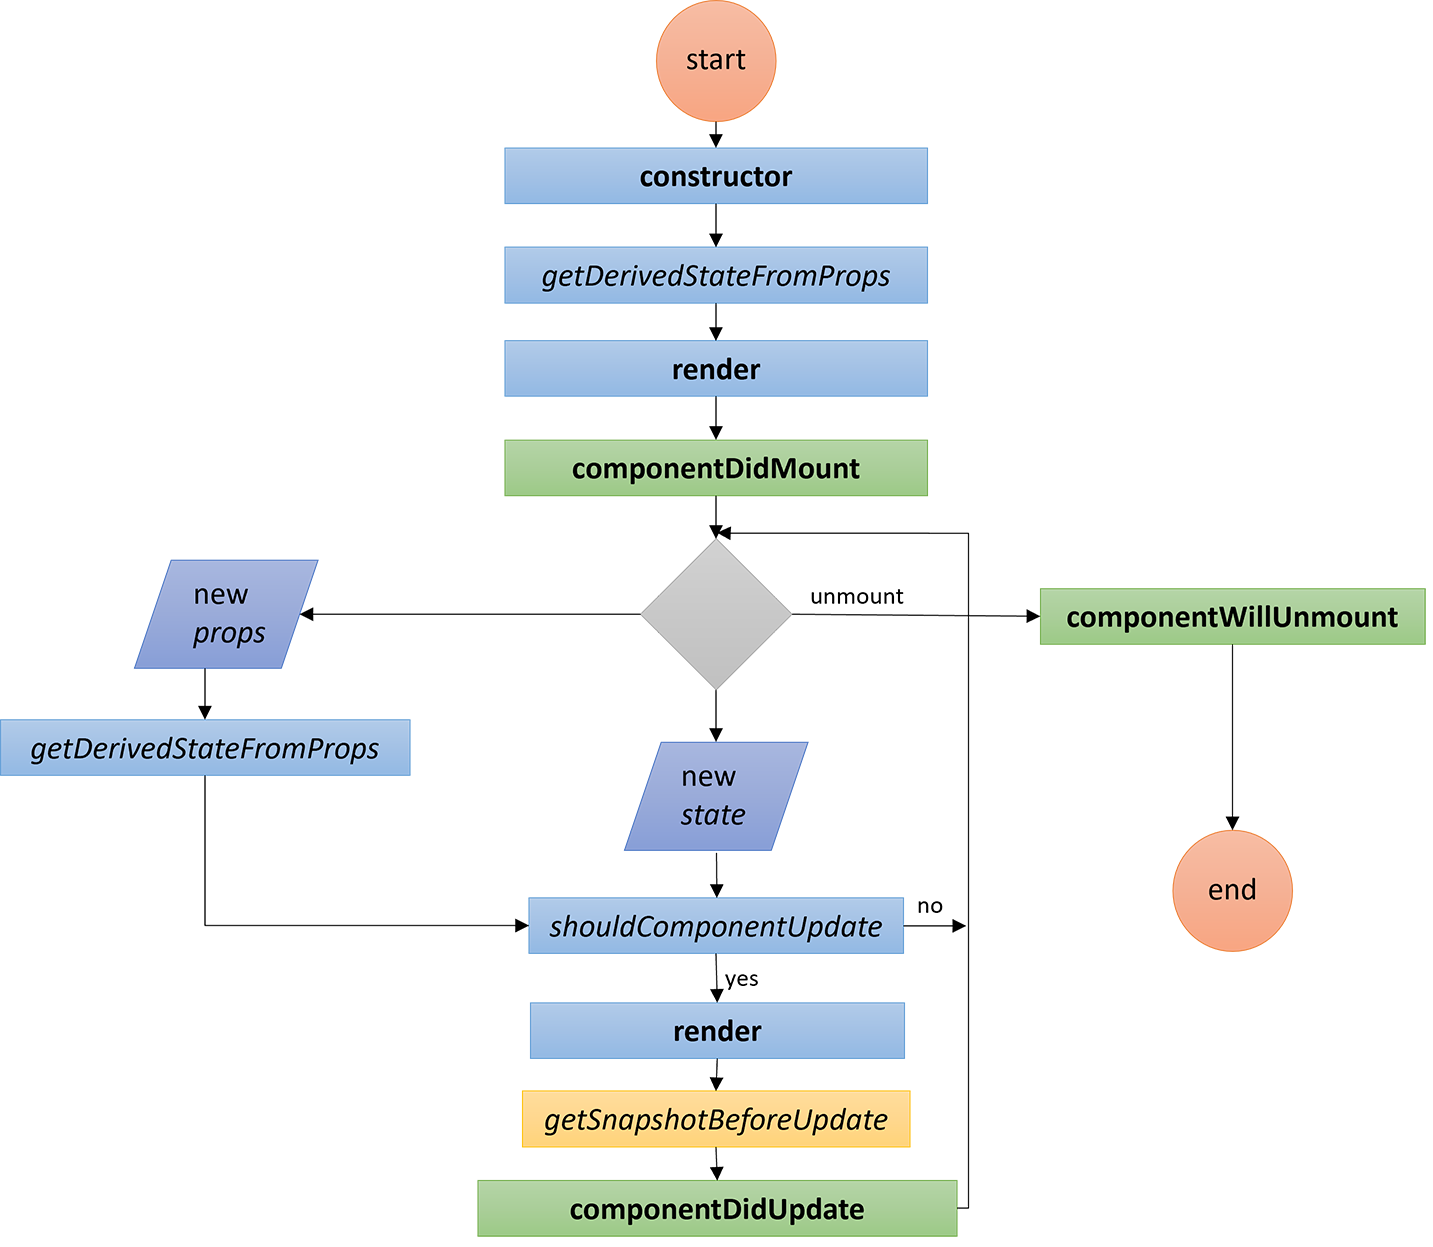
\includegraphics[width=\textwidth]{images/react_component_lifecycle_flu.png}
        \caption{Diagrama de flujo de un componente en React.}
        \label{fig::react_component_lifecycles_flu}
    \end{figure}
    
    Ya visto el ciclo de vida de un componente en React y los diferentes métodos y procedimientos que se utilizan para la creación y renderización en cada uno de ellos, podemos observar que la estructura de un componente equivale a la clásica definición de \textit{clase} utilizada en la programación orientada objetos, la cuál se implementa en otros lenguajes como en el caso de \textit{Java}, donde cada objeto tiene una serie de atributos (que corresponde al estado local) que se inicializan en su respectivo método constructor utilizando unos valores por defecto (las \textit{props} dadas al crear la referencia del componente) y una serie de métodos que permiten actualizar e interactuar con sus atributos. Sin embargo, en las últimas versiones de ReactJS; concretamente a partir de la versión 16.8, se introduce un nuevo concepto en la programación de estos componentes llamado \textbf{hook}. Aunque la lógica sigue siendo la misma y en lenguaje base del \textit{framework} también, esta nueva definición se encarga de sustituir la estructura clásica de un componente basada en el uso de clases por la división del mismo en funciones atómicas. 
    
    Cuando un componente crece en complejidad también lo hace el número de funciones declaradas, cada una con un propósito diferente. Supongamos que en el \textit{state} del componente tenemos un atributo llamado \textit{contador} que indica el número de usuarios que han visitado nuestra web y que, para actualizarlo, usamos un botón que haga una petición a una API. Utilizando la definición de clase, el código implementado quedaría algo parecido a como se muestra en la figura \ref{fig::estructura_contador_clase}. \\

    \begin{figure}[!h]
        \centering
        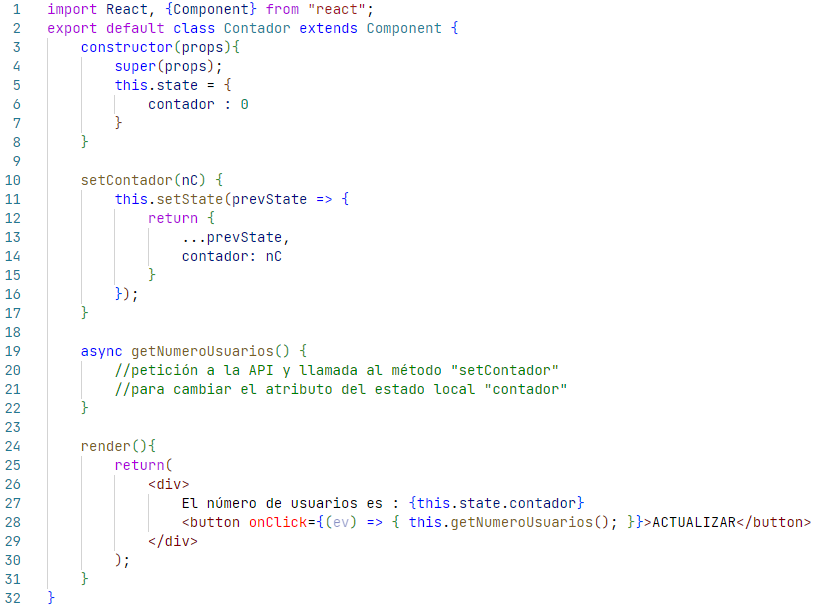
\includegraphics[width=\textwidth]{images/componente_estructura_clase.PNG}
        \caption{Componente ``Contador'' con clases.}
        \label{fig::estructura_contador_clase}
    \end{figure}
    
    Si por el contrario decidimos de utilizar la definición de \textit{hook} de un componente, recurriremos entonces a las funciones de JavaScript para su implementación. El contenido de estas funciones será el siguiente: 
    
    \begin{itemize}
        \item Lo primero es la creación de las constantes que hagan referencia tanto a los atributos como a sus métodos correspondientes que actualicen el valor. Por defecto, estas se crean nombrandolas y referenciándolas a \textit{useState}; aunque pueden modificarse para que hagan más operaciones. Esto hace referencia al constructor.
        
        \item A continuación deberán de definirse todas aquellas funciones y métodos que se encargan tanto del procesamiento de datos como de la llamada a APIs. 
        
        \item Como toda función, esta debe de retornar algo, y este caso, es la vista del componente utilizando JSX. Desempeña el mismo papel que la función \textit{render}. \\
        
        \begin{figure}[!h]
            \centering
            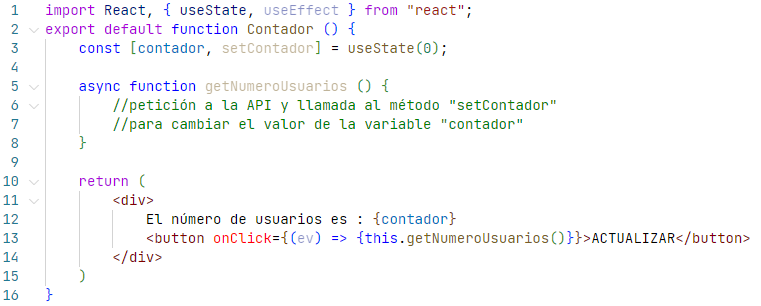
\includegraphics[width=\textwidth]{images/componente_estructura_hook.PNG}
            \caption{Componente ``Contador'' con hooks.}
            \label{fig::estructura_contador_hooks}
        \end{figure}
        
    \end{itemize}
    
    Con esto damos por finalizado el estudio de las tecnologías a utilizar en la implementación de las simulaciones, por lo que en el siguiente capítulo continuaremos con su programación, utilizando para ello las expresiones de la tabla \ref{tab:ecuaciones_todas}.\\

\end{document}